\section{Catalyst}
\label{sec:Catalyst}

Although it is straightforward for a simulation development team to add some
basic \vda capabilities into simulation code, our desire is to have a
general-purpose fully-featured library that leverages existing
implementations.  The intention is threefold.  First, by leveraging existing
\vda libraries we can benefit from the accumulation of over two decades of
visualization research and development.  Second, by making the library
general purpose we can quickly apply our \insitu \vda capabilities to many
simulations as opposed to a single simulation.  Third, by using our
existing code we can integrate the \insitu tools with our traditional
post-processing tools both to provide interfaces that users are already
familiar and comfortable with and to apply scalable algorithms designed for
\insitu with our post-processing tools and vice versa.

Catalyst is a C++ library with an externally facing API to C, FORTRAN, and
Python.  It is built atop the Visualization Toolkit (VTK)\lcite{VTK} and
ParaView\lcite{ParaView}.  By building Catalyst with VTK, it can access a
large number of algorithms including writers for I/O, rendering algorithms,
and processing algorithms such as isosurface extraction, slicing, and flow
particle tracking.  Catalyst uses ParaView to implement and manage the
\vda, which is defined using a visualization
pipeline\lcite{Moreland2013:TVCG}.  Although it is possible to construct
pipelines entirely in C++, the ParaView control structure allows pipelines
configured through Python scripts.

\begin{figure}[htb]
  \centering
  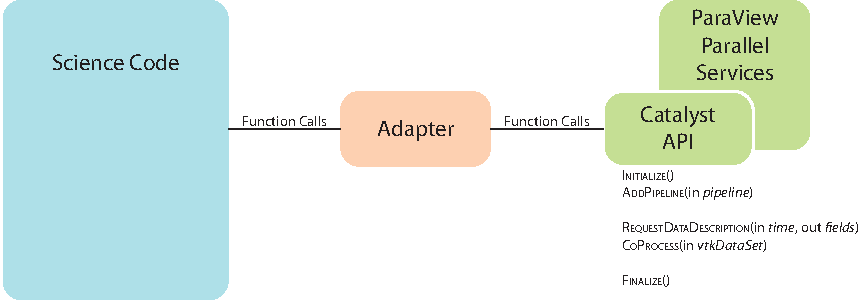
\includegraphics{figures/CatalystCoupling}
  \caption{Coupling a simulation with Catalyst.}
  \label{fig:CatalystCoupling}
\end{figure}

Since Catalyst will extend to a variety of existing simulation codes, our
design does not expect its API to easily and efficiently process internal
structures in all possible codes directly.  Our solution is to rely on
adapters --- which are small pieces of code written for each new linked
simulation --- to translate data structures between the simulation's code
(for our use case the CTH shock physics code) and Catalyst's VTK-based
architecture, as shown in Figure~\ref{fig:CatalystCoupling}.  The adapter
must also establish a mechanism that allows the simulation to define a
visualization pipeline and periodically invoke the analysis while running
the simulation, which in our CTH adapter we control through the CTH input
deck.

To conserve memory, our adapter directly interfaces the \vda code to the
data structures defined by CTH.  This interface is challenging because
although the blocks of data are represented sequentially in both CTH and
VTK, the multidimensional order is different.  To address this, our adapter
contains an interface wrapper above the standard VTK array.  The wrapper
reimplements the array's accessor functions to handle the order difference
between the two systems.  Although there is a minor overhead in additional
pointer arithmetic and virtual method calls, it saves us from a deep memory
copy.

The Catalyst library and the algorithms we use within CTH are an
accumulation of several years work, starting with the development of
fragment analysis algorithms with our post-processing
tools\lcite{Moreland2008:UltraVis,Ice2009,Moreland2010}, described in more
detail in Section~\ref{sec:UseCase}.  Subsequent work lead to the
development of Catalyst\lcite{Fabian2011} and the scaling of algorithms
used in conjunction with CTH\lcite{Fabian2012}.
